O objetivo principal do agente de \textit{MM} é decidir dentro do intervalo de preços possíveis para o ativo o que proporcione um maior retorno financeiro para o menor risco associado, de acordo com a fronteira eficiente de execução ótima \citep{almgren2000}. O agente também pode decidir a quantidade $Q$ de ações ofertadas por determinado preço $p$, mas não tem controle direto sobre as quantidades efetivamente negociadas. Ou seja, a quantidade executada $N \leq Q$ é uma variável aleatória, dado que não é possível determinar de antemão quanto o agente agressor irá negociar com o agente de \textit{market-making} \citep{rao2020stochastic}.

É possível representar essa dinâmica na forma de um problema de otimização estocástica com restrições, onde o objetivo do agente (ou controle) consiste em obter uma aproximação ótima da equação de valores-estados de Bellman $Q^*(s, a) = \mathbb{E} \left[ R_{t+1} + \gamma \cdot \max_{a'} Q^*(S_{t+1}, a') \mid S_t = s, A_t = a \right]$ para um processo de decisão de Markov (ou \textit{Markov Decision Process} em inglês). Para processos com ambientes mais simples é possível obter soluções analíticas, como proposto por \citep{Avellaneda2008} e \citep{rao2020stochastic} para intervalos de tempo contínuo. Existem métodos numéricos iterativos, que consistem em aproximar os valores das probabilidades de transição da política (\textit{policy-iteration}) ou da função valor (\textit{value-iteration}) por iterações consecutivas no ambiente.

\begin{itemize}
	\item \textbf{Aprendizado por Reforço - Temporal Difference Learning:}
	\begin{itemize}
		\item O TD learning é uma técnica de aprendizado por reforço que visa aprender a função valor de um estado ou ação de forma incremental com base nas diferenças temporais entre as estimativas sucessivas.
		\item A atualização típica do TD learning para um estado \(s\) é dada por \(V(s) \leftarrow V(s) + \alpha \cdot (R + \gamma \cdot V(s') - V(s))\), onde \(R\) é a recompensa imediata, \(\gamma\) é o fator de desconto, \(s'\) é o próximo estado, e \(\alpha\) é a taxa de aprendizado.
	\end{itemize}
	
	\item \textbf{Aprendizado por Reforço - Q-Learning:}
	
	\begin{itemize}
		\item O Q-Learning é um método de aprendizado por reforço que visa aprender a função Q, que representa a qualidade de tomar uma ação específica em um determinado estado.
		\item A regra de atualização típica do Q-valor é \(Q(s, a) \leftarrow Q(s, a) + \alpha \cdot (R + \gamma \cdot \max_{a'} Q(s', a') - Q(s, a))\), onde \(s'\) é o próximo estado, \(R\) é a recompensa, \(\gamma\) é o fator de desconto e \(\alpha\) é a taxa de aprendizado.
	\end{itemize}
	
	\item \textbf{Aprendizado por Reforço - Actor-Critic Learning:}
	
	\begin{itemize}
		\item O AC-learning envolve duas partes principais: o crítico (critic) que avalia as ações, e o ator (actor) que escolhe as ações. O objetivo é otimizar a política do ator com base nas avaliações do crítico.
		\item O crítico aprende uma função de valor como no TD learning, enquanto o ator atualiza a política para maximizar os valores de ação estimados pelo crítico.
	\end{itemize}
	
	\item \textbf{Aprendizado por Reforço - Deep Q-Learning (DQL):}
	
	\begin{itemize}
		\item O DQL é uma extensão do Q-Learning que incorpora redes neurais profundas para lidar com espaços de estados e ações contínuos ou de alta dimensionalidade.
		\item \textbf{Redes Neurais:} A função Q é aproximada por uma rede neural profunda. O algoritmo utiliza a experiência passada armazenada em um buffer de repetição para realizar atualizações mais estáveis.
		\item A atualização do Q-valor torna-se \(Q(s, a) \leftarrow Q(s, a) + \alpha \cdot (R + \gamma \cdot \max_{a'} Q(s', a'; \theta^-) - Q(s, a; \theta))\), onde \(\theta\) são os parâmetros da rede neural, e \(\theta^-\) representa os parâmetros da rede no passo anterior.
	\end{itemize}
\end{itemize}

Técnicas mais simples para obter políticas com retorno ótimo requerem um modelo perfeito do ambiente, ou então necessitam de grande uso de memória para armazenar valores de Q intermediários, mas o uso de redes neurais para aproximar os valores de Q são uma solução eficiente para minimi

\begin{itemize}
	\item Trajetória ($\tau$): é a sequência de estados observados e ações tomadas ao longo do tempo. No contexto de \textit{MM}, uma trajetória consiste em uma série de estados do mercado $s_{t} = (o_{t}, L_{t})$ seguidas da ação em cima desse estado $a_{t} = \{(\delta_{t}(p_{i}), Q_{i}) \ | \ \forall i \}$. Essas trajetórias representam a jornada do agente no mercado financeiro, incluindo suas ações e interações com o ambiente.
	
	\[
	\tau = (s_0, a_0, s_1, a_1, \ldots, s_T, a_T)
	\]
	
	Onde \(s_t\) é o estado no tempo \(t\), e \(a_t\) é a ação tomada no tempo \(t\).
	
	\item Política ($\pi$): função que mapeia o estado atual (\textit{spreads} $\delta$ e quantidades $Q$) para a escolha de ações (ofertas de compra e venda). Através de algoritmos de otimização de decisão (\textit{Policy Optimization} e \textit{Q-Learning}), nosso objetivo é encontrar uma política ótima que permita ao agente tomar decisões que maximizem seus retornos no mercado. Essa política é fundamental para determinar como o agente se comporta em diferentes situações de mercado.
	
	\[
	\pi(s) \rightarrow a
	\]
	
	Essa função determina como o agente toma decisões em diferentes estados.
	
	\item Função de Ação-Valor ($Q$): estima o valor esperado acumulado que o agente pode obter tomando a ação $a$ e em sequência seguir a política \(\pi\) a partir de um estado inicial $s$. No contexto do agente de \textit{Market Making}, $Q$ depende do preço de venda $p$ e da quantidade $N$ executada, bem como da política do agente. Através do Aprendizado por Reforço, podemos obter $V$ \(Q\) e obter $V$ a  para avaliar quão bom é um estado, o que orienta o agente na seleção de ações que maximizam seu desempenho global.
	
	\begin{equation*}
		V(s_0) = \mathbb{E}\left[\sum_{t=0}^{T} \gamma^t \cdot r(s_t, \pi(s_t)) \right]
		\end{equation*}
	
	Onde $\gamma$ é o fator de desconto que pondera as recompensas futuras e geralmente $0 < \gamma \leq 1$. A função valor considera a expectativa de retorno sobre todas as possíveis trajetórias do agente.
\end{itemize}

\begin{figure}[H]
	\centering
	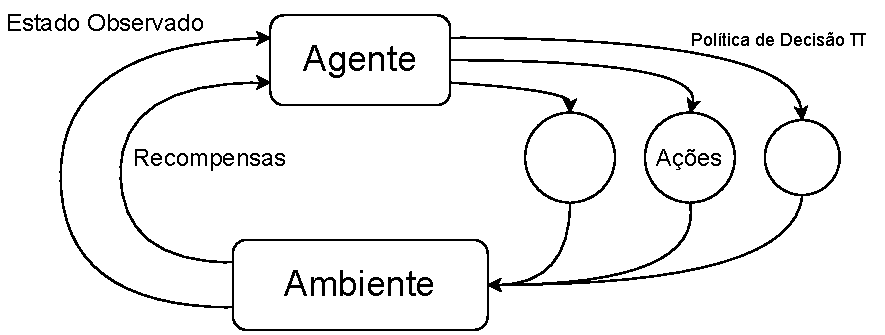
\includegraphics{files/rl-agent.pdf}
	\caption{Autômato do Agente sob o paradigma de Aprendizado por Reforço}
	\label{fig:rl-agent}
\end{figure}

O problema passa a ser representado pela nova tupla $(V, \tau, \pi)$ onde $V$ e $\tau$ são observados como saída do ambiente. O paradigma de Aprendizado por Reforço permite que o agente se adapte a mudanças nas condições de mercado ao longo do tempo, e que a política escolhida considere o impacto das transações do próprio agente sobre o mercado, tornando-o mais resiliente a flutuações causadas pelas próprias ações. Uma vez treinado, o agente pode ser usado para tomar decisões em tempo real no mercado financeiro, proporcionando uma vantagem competitiva para instituições financeiras e o avanço da pesquisa em finanças quantitativas e aprendizado de máquina, abrindo novas possibilidades para o desenvolvimento de estratégias de negociação mais eficientes e robustas. A contribuição da pesquisa proposta será tornar o agente adverso ao risco noturno, inserindo-se também uma restrição adicional, de que ao final do dia não haja exposição a riscos de mercado. 
Existem algumas alternativas para formalizar matematicamente essa restrição:
\begin{enumerate}
    \item No final do dia, o agente não pode ter nenhum ativo em posição: 
    \begin{equation} \label{overnight_restriction}
        \sum_{i = 0}^{n} q_{T, i}^{a}  = \sum_{i=0}^{m} q_{T, i}^{b} = 0
    \end{equation}
    \item No final do dia, se houver alguma posição restante, o agente precisa \textit{headgear}\footnote{De maneira simplificada, o \textit{hedge} consiste em comprar ou vender ativos que tenham uma exposição ao risco oposta aos riscos da carteira atual, de modo a equilibrar a posição.} sua exposição ao risco ao participar em outros mercados abertos no momento, abordagem que chamamos de \textit{market making} \textbf{simultâneo}.
\end{enumerate}
